%% rules definition for the listing package
\lstset{ %
  backgroundcolor=\color{white},   % choose the background color; you must add \usepackage{color} or \usepackage{xcolor}; should come as last argument
  basicstyle=\footnotesize,        % the size of the fonts that are used for the code
  breakatwhitespace=false,         % sets if automatic breaks should only happen at whitespace
  breaklines=true,                 % sets automatic line breaking
  captionpos=b,                    % sets the caption-position to bottom
  commentstyle=\color{black},      % comment style
  deletekeywords={...},            % if you want to delete keywords from the given language
  escapeinside={\%*}{*)},          % if you want to add LaTeX within your code
  extendedchars=true,              % lets you use non-ASCII characters; for 8-bits encodings only, does not work with UTF-8
  frame=single,	                   % adds a frame around the code
  keepspaces=true,                 % keeps spaces in text, useful for keeping indentation of code (possibly needs columns=flexible)
  keywordstyle=\color{black},       % keyword style
  language=bash,                 % the language of the code
  morekeywords={*,...},            % if you want to add more keywords to the set
  numbers=left,                    % where to put the line-numbers; possible values are (none, left, right)
  numbersep=5pt,                   % how far the line-numbers are from the code
  numberstyle=\tiny\color{black},  % the style that is used for the line-numbers
  rulecolor=\color{black},         % if not set, the frame-color may be changed on line-breaks within not-black text (e.g. comments (green here))
  showspaces=false,                % show spaces everywhere adding particular underscores; it overrides 'showstringspaces'
  showstringspaces=false,          % underline spaces within strings only
  showtabs=false,                  % show tabs within strings adding particular underscores
  stepnumber=1,                    % the step between two line-numbers. If it's 1, each line will be numbered
  stringstyle=\color{black},       % string literal style
  tabsize=2,	                   % sets default tabsize to 2 spaces
  title=\lstname                   % show the filename of files included with \lstinputlisting; also try caption instead of title
}

\section{Panoramica e utilizzo del sistema}

Il sistema è formato da un client VNC in esecuzione sul Raspberry Pi 2, a sua volta collegato attraverso un cavo HDMI ad un proiettore.  Si utilizza un meccanismo di connessione chiamato \textit{reverse connection}, tipicamente è il client ad iniziare una connessione verso un server; in questo caso invece il client resta in ascolto in attesa di connessioni ed è il server VNC che viene mandato in esecuzione su un laptop all'inizio di ogni proiezione a richiedere il collegamento.

\begin{figure}[h!]
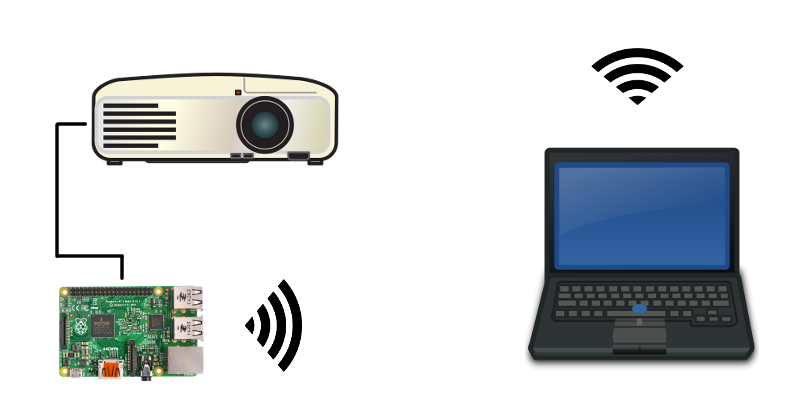
\includegraphics[width=12cm, height=6cm]{../img/setup}
\centering
\caption{Raspberry Pi projector: panoramica del setup}
\end{figure}

\paragraph{Scenari d'uso}
È possibile definire una descrizione di un caso d'uso tipico del sistema, da parte di un utente che sia ad esempio un relatore ad una conferenza pubblica o un professore universitario durante una lezione in aula, che utilizza comunemente il proiettore come supporto su cui mostrare delle slide o appunti che aiutino gli studenti a seguire le lezioni.\\
Inizialmente, il laptop personale dell'utente dovrà essere configurato seguendo un tutorial, che segue i passi descritti nelle sezioni successive, ampliandone i dettagli e che sarà reso disponibile dall'amministratore del sistema.\\
La configurazione servirà ad installare il software necessario, e sarà obbligatoria solo al primo utilizzo, dopodiché basterà eseguire il server VNC per avere il proiettore wireless pronto all'uso.\\
Il Raspberry Pi 2 dovrà essere collegato al proiettore e già acceso al momento in cui il laptop apre la connessione VNC. \\

\section{Configurazione del server}
Il procedimento con cui si è configurato il server VNC differisce con il sistema operativo utilizzato.
\subsection{Windows}
Su sistema operativo Windows 10 è stato installato e configurato il software TightVNC rilasciato con licenza GPL2 nella versione non commerciale.
Dopo l'installazione il programma è già in esecuzione e si può procedere alla configurazione:
facendo clic con il tasto destro sull'icona del TightVNC Server nella system tray, apparirà una finestra popup nella quale sarà sufficiente selezionare la voce "Attach Listening Viewer".

\begin{figure}[h]
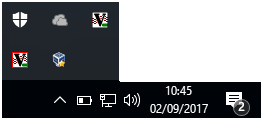
\includegraphics[width=8cm]{../img/tightvncserver1}
\centering
\caption{TightVNC Server: Icona (rossa) del TightVNC Server nella system tray}
\end{figure}

\begin{figure}[h]
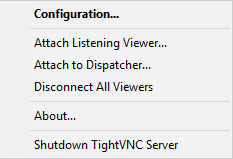
\includegraphics[width=8cm]{../img/tightvncserver2}
\centering
\caption{TightVNC Server: Opzioni visualizzabili con clic destro su icon tray}
\end{figure}

Comparirà un'ulteriore finestra, nella quale sarà possibile specificare un indirizzo e una porta TCP per un client in ascolto.

\begin{figure}[h] %here
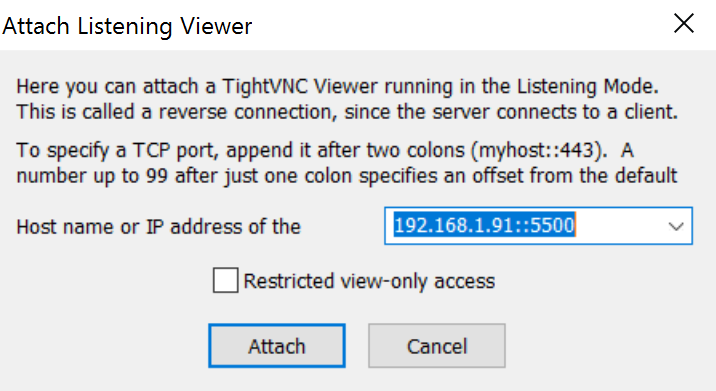
\includegraphics[width=8cm]{../img/tightvncserver3}
\centering
\caption{TightVNC Server: Attach Listening Viewer}
\end{figure}

Fare tick su "Restricted view-only access" per evitare che il client possa agire modificando il desktop del server.
Se viene rilevato un client in listening all'indirizzo specificato, viene avviata immediatamente la condivisione dello schermo.

È stato inoltre aggiunto un hostname nel file \textit{C:\textbackslash Windows \textbackslash system32\textbackslash drivers\textbackslash etc \textbackslash hosts} per identificare il Raspberry Pi 2 all'interno della sottorete.\newpage

Con TightVNC è possibile limitare la porzione di schermo da virtualizzare utilizzando una delle opzioni del pannello di configurazione, o in alternativa, da linea di comando usando
\begin{lstlisting}
tvnserver.exe -sharerect widthxheight+left+top
\end{lstlisting}
considerando che l'origine (0,0) del piano è posizionata all'angolo in alto a sinistra del display primario.

\begin{figure}[h]
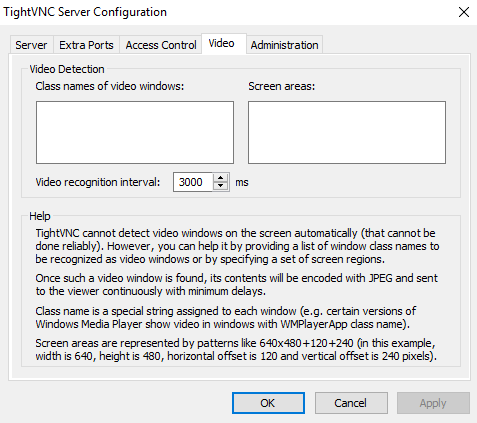
\includegraphics[width=8cm]{../img/tightvncserver4}
\centering
\caption{TightVNC Server: Screen areas}
\end{figure}

\subsection{macOS}
Su sistema operativo macOS Sierra si è utilizzato il software Vine Server (OSXvnc), che è open source e distribuito con licenza GPL3.

\begin{figure}[h!]
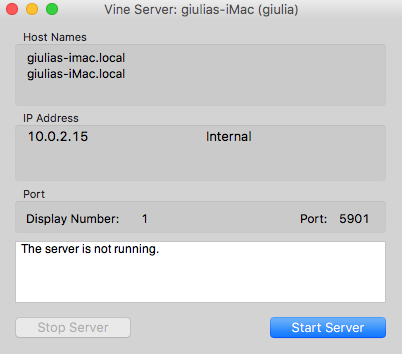
\includegraphics[width=8cm]{../img/vine1}
\centering
\caption{Vine Server: schermata principale}
\end{figure}

\begin{figure}[h!]
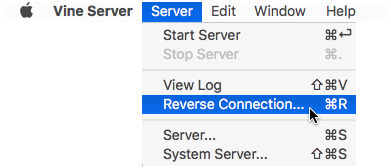
\includegraphics[width=8cm]{../img/vine2}
\centering
\caption{Vine Server: configurazione con reverse connection}
\end{figure}

\subsection{GNU/Linux}
Il testing è avvenuto su distribuzione Ubuntu alla versione 16.04 Xenial Xerus.

\paragraph*{x11vnc}
\noindent È un server VNC ricco di funzionalità e possibilità di personalizzazione, facilmente acquisibile perché presente come package nei repository ufficiali:
% listing
\begin{lstlisting}
sudo apt-get install x11vnc
\end{lstlisting}

\noindent Una connessione viene istanziata dal server x11vnc lanciando semplicemente il comando
\begin{lstlisting}
x11vnc -connect <client-ip-address>:<port>
\end{lstlisting}
con cui il server si collega al client in listening mode specificato da indirizzo e porta TCP.\\

Con x11vnc è inoltre possibile modificare la risoluzione del pannello VNC per adattarla a quella del proiettore in modo da ottenere la visione migliore. \\
È possibile infatti usare l'opzione \textit{-geometry WxH} oppure l'opzione \textit{-scale factor} per specificare nel primo caso larghezza ed altezza in pixel, e nel secondo un fattore con cui scalare il framebuffer.

\begin{lstlisting}
x11vnc -geometry 1600x1200
x11vnc -scale 0.8
\end{lstlisting}

Un'altra opzione utile è \textit{-clip WxH+X+Y}, che consente di ridurre l'area di schermo da visualizzare sul client. Questa opzione può essere combinata con le precedenti per riadattare la risoluzione dello schermo una volta applicato il ridimensionamento del pannello.

\begin{lstlisting}
x11vnc -clip 800x600+0+0 -geometry 1920x1080
\end{lstlisting}

Anche in questo caso è possibile aggiungere un hostname che identifichi il Raspberry Pi 2 all'interno della sottorete, è sufficiente modificare (con privilegi da amministratore) il file /etc/hosts aggiungendo la linea

\begin{lstlisting}
192.168.1.78    raspberrypi.localdomain raspberrypi
\end{lstlisting}

avendo sostituito all'indirizzo quello corrente del client.\\

\subsection{Android/iOS}
Sebbene fosse inizialmente tra gli obiettivi del progetto quello di includere tra i sistemi operativi supportati anche quelli mobili - data la crescente diffusione di questi ultimi anche nel supporto di presentazioni pubbliche - date le molte difficoltà incontrate, non si sono trovate soluzioni soddisfacenti.\\
In Android sono presenti o soluzioni parziali come server che non supportano reverse connection, oppure soluzioni che richiedono il rooting del dispositivo da parte dell'utente.\\
In iOS l'unico server disponibile (Veency) è utilizzabile solo da chi ha effettuato il jailbreak del proprio dispositivo, e d'altra parte Apple non sembra interessata a supportare VNC anche in mobile, dove per la condivisione in remoto di contenuti è già disponibile la suite AirPlay.
%% aggiungi alla sitografia http://lowendmac.com/2013/what-does-apple-have-against-vnc-server-on-ios/
\section{Configurazione del client}
Il Raspberry Pi 2 è dotato di sistema operativo Raspbian, basato su distribuzione Debian nella sua versione per architetture ARM. \\
La configurazione del client può essere suddivisa in sottosezioni.
\subsection{Startup del VNC client all'avvio}
Considerando che il Raspberry Pi 2 viene utilizzato come dispositivo headless - senza tastiera e mouse collegati - è necessario che dopo il setup iniziale, ogni programma venga avviato in modo automatico. Per abilitare il client all'avvio è stato utilizzato un metodo che si avvale di desktop entry e della presenza di X in corretta esecuzione.\\
È un metodo supportato dai maggiori \textit{desktop environment}, tra i quali LXDE e il suo derivato PIXEL, disponibile in Raspbian.

\noindent È necessario innanzitutto abilitare il boot con il desktop
\begin{lstlisting}
sudo raspi-config
\end{lstlisting}

\noindent Selezionando
\begin{verbatim}
Enable boot to desktop/Scratch >
Desktop Log in as user ‘pi’ in the graphical desktop .
\end{verbatim}

\noindent Dopodiché creiamo un file .desktop (o desktop entry) nella directory usata dall'ambiente desktop per l'autostart delle applicazioni; quella di default, a livello utente è \textit{~/.config/autostart/}:
\begin{lstlisting}
cd /home/pi/.config
mkdir autostart
cd autostart
nano tightvnc.desktop
\end{lstlisting}

Scrivendo nel file di configurazione:

\begin{lstlisting}
[Desktop Entry]
Type=Application
Name=TightVNC
Exec=vncviewer -viewonly -fullscreen -listen
StartupNotify=false
\end{lstlisting}

Tramite il campo Exec viene specificato il comando da eseguire all'avvio.\\
In questo modo il VNC viewer sarà messo in ascolto ed eseguito senza che possa modificare il desktop del server e in modalità a schermo intero.

\noindent Infine è necessario salvare e riavviare per apportare le modifiche
\begin{lstlisting}
sudo reboot
\end{lstlisting}

\subsection{Indirizzo IP statico}
La configurazione di un indirizzo IP (privato) statico sul client è utile per fare in modo che i server conoscano in anticipo l'indirizzo del client, prevedendo che comunque il Raspberry Pi sia utilizzato sempre nella stessa sottorete.\\
È necessario modificare /etc/dhcpcd.conf, il file di configurazione letto dal demone di \textit{dhcpcd}, un client DHCP e DHCPv6 open source.

\begin{lstlisting}
interface wlan0
static ip_address=192.168.1.78/24
static routers=192.168.1.254
static domain_name_servers=192.168.1.254

\end{lstlisting}

\subsection{Disabilitare il blank screen}
Questo passo è necessario per evitare che il desktop grafico del Raspberry vada in standby interrompendo la presentazione. \\
È sufficiente modificare il file di configurazione del display manager (LightDM) \textit{/etc/lightdm/lightdm.conf} aggiungendo nella sezione [SeatDefaults] il comando
\begin{lstlisting}
[SeatDefaults]
xserver-command=X -s 0 -dpms
\end{lstlisting}

\subsection{Streaming audio e video}

%%PULSEAUDIO, PULSEAUDIO OVER THE NETWORK
\paragraph*{PulseAudio}
È un server audio che funge da proxy per tutte quelle applicazioni che utilizzano l'audio tramite componenti come ALSA e OSS.
Una delle caratteristiche più interessanti di PulseAudio è che può essere utilizzato via rete per fare streaming audio da un client ad un server sul quale è in esecuzione il demone PulseAudio, permettendo la riproduzione del suono sul server.\\

Per prima cosa è necessario abilitare lo streaming attraverso TCP per client anonimi.\\

\noindent Nel file di configurazione /etc/pulse/default.pa abilitare i seguenti parametri sul server (Pi):
\begin{lstlisting}
load-module module-native-protocol-tcp auth-ip-acl=127.0.0.1;192.168.0.0/24 auth-anonymous=1
\end{lstlisting}

Dove la sottorete LAN (192.168.0.0/24) deve coincidere con quella in cui si trovano i client che richiedono di connettersi.

\noindent Sul client (laptop), aggiungere la riga
\begin{lstlisting}
load-module module-native-protocol-tcp
\end{lstlisting}

Successivamente, per fare in modo che il server PulseAudio compaia nel PulseAudio Device Chooser (pasystray), si devono caricare i moduli zeroconf necessari e abilitare il demone Avahi.

\noindent Sia sul server che sul client
\begin{lstlisting}
sudo apt install pulseaudio-module-zeroconf
sudo systemctl start avahi-daemon.service
sudo systemctl enable avahi-daemon.service
\end{lstlisting}


\noindent Sul server, in /etc/pulse/default.pa è necessario aggiungere la riga
\begin{lstlisting}
load-module module-zeroconf-publish
\end{lstlisting}


\noindent Mentre sul client, in /etc/pulse/default.pa
\begin{lstlisting}
load-module module-zeroconf-discover
\end{lstlisting}

Ora per ridirezionare un qualsiasi stream o output audio al server PulseAudio remoto è sufficiente selezionare il sink appropriato ad esempio utilizzando PulseAudio Volume Control (pavucontrol).\\
%% INSERISCI IMMAGINE PAVUCONTROL
Se non appaiono i sinks sul client, provare a riavviare il demone Avahi sul server per rifare il broadcast delle interfacce disponibili.
\begin{lstlisting}
sudo systemctl restart avahi-daemon.service
\end{lstlisting}
\begin{comment}
\noindent Altri comandi utili per riavviare PulseAudio in caso di errore
\begin{lstlisting}
pulseaudio -k
pulseaudio -D
\end{lstlisting}
\end{comment}

%È INSTABILE, purtroppo non ho trovato una soluzione, ne scriverò nelle valutazioni e miglioramenti
% così aggiunge un tunnel, è un'altra cosa
% ho provato ad aggiungere la linea
% load-module module-tunnel-sink server 192.168.1.73 sink_name=Pi2
% sul laptop

%% eseguire pulseaudio con flag -vvv per avere più info...è incredibile che dopo aver cambiato il volume diventi stabile! sinceramente mi viene il dubbio che sia il laptop il problema.
% testato collegando il laptop in ethernet, si blocca ancora, sembra un po' casuale il tempo che intercorre tra un blocco e un altro, dopo un po' di prove sembra essersi stabilizzato
%% posso pensare ad una patch in cui ad ogni secondo si alza e si riabbassa il volume in modo che il sink resti sempre attivo
%Nel caso il suono si blocchi, spesso basta riavviare il demone PulseAudio sul server: (è instabile) oppure semplicemente alzare/diminuire il volume del sink (da impostazioni audio in shortcut, non da pavucontrol)! ma perché!


\subsection{File system read-only}
%% INTRODUZIONE, CONSIDERAZIONI FILE SYSTEM READONLY, UTILITÀ, PERCHÉ USARE UNION-FS , ETC
%% TODO AGGIUNGI IN SITOGRAFIA IL TIZIO
Prevedendo un utilizzo continuativo del Raspberry Pi, e non potendo assicurarsi sempre un corretto spegnimento del dispositivo, è stato necessario trovare un metodo che potesse limitare al minimo i rischi di danneggiare la micro SD sulla quale il sistema è installato. \\
Una delle soluzioni è quella di minimizzare le scritture su memoria SD, che potrebbero lasciare il file system in uno stato incoerente ad esempio in caso di repentini cali di tensione o spegnimenti erronei. \\ A tale scopo, si è predisposto un meccanismo che rende possibile l'utilizzo in read-only delle partizioni sensibili (di sistema) e garantisce comunque la possibilità di mantenere e amministrare il sistema stesso perché consente uno switch in read-write ogni volta che l'amministratore debba installare nuovi programmi o apportare modifiche nei file di configurazione.

\paragraph*{UnionFS}
È un file system Linux che permette \textit{union mount}, ovvero consente di simulare l'unione di più file system sottostanti. File e directory in file system separati, denominati \textit{branch} vengono sovrapposti in modo trasparente, determinando un unico file system coerente.\\
I diversi branch possono essere sia in sola lettura che in scrittura e lettura: in questo caso le scritture nella copia unificata vengono indirizzate verso uno specifico e reale file system. Questo permette ad un file system di apparire come scrivibile anche se in realtà non lo è. \\
Un esempio di utilizzo di questo particolare meccanismo (\textit{copy-on-write}) si ha nei Live CD. \\
Nel progetto è stato utilizzato unionfs-fuse, una implementazione userspace di UnionFS, che presenta la stesse caratteristiche.\\
È stato utilizzato per sovrapporre ad un sistema in sola lettura, un file system temporaneo memorizzato in RAM; ciò comporta che ogni scrittura effettuata avvenga in RAM e non nella memoria SD, con conseguente perdita di ogni informazione aggiunta ad ogni riavvio del Raspberry.\\ In questo modo si previene che eventuali scritture possano danneggiare o modificare il file system in modo inappropriato.

\noindent unionfs-fuse è disponibile come pacchetto nei repository di Raspbian:
\begin{lstlisting}
apt-get update
apt-get install unionfs-fuse
\end{lstlisting}

\noindent È necessario disabilitare tutti i servizi che possono scrivere in modo
incontrollato su micro SD, tra i quali anche il servizio che si occupa della memoria swap:
\begin{lstlisting}
dphys-swapfile swapoff
dphys-swapfile uninstall
update-rc.d dphys-swapfile disable

systemctl disable systemd-readahead-collect
systemctl disable systemd-random-seed

\end{lstlisting}

\noindent Inoltre creiamo uno script per potere utilizzare UnionFS:
\begin{lstlisting}
touch /usr/local/bin/mount_unionfs
chmod +x /usr/local/bin/mount_unionfs
nano /usr/local/bin/mount_unionfs

\end{lstlisting}

\noindent In cui scriveremo

\begin{lstlisting}
#!/bin/sh
 DIR=$1
 # check if root is rw or ro
 ROOT_MOUNT=$(awk '$2=="/" {print substr($4,1,2)}' < /etc/fstab)
 if [ $ROOT_MOUNT = "rw" ]
 then # remount the first directory in the second
   /bin/mount --bind ${DIR}_org ${DIR}
 else
   # remount the directory as tmpfs or ramdisk
   /bin/mount -t tmpfs ramdisk ${DIR}_rw
   /usr/bin/unionfs-fuse -o cow,allow_other,suid,dev,nonempty ${DIR}_rw=RW:${DIR}_org=RO ${DIR}
 fi
\end{lstlisting}
% cow: enables copy on write
% allow_other: allow access to other users
% suid:
% dev:
% nonempty: allow mounts over nonempty files/dir
% l'ultimo pezzettino specifica come fare il mergin delle directory
% es. root_rw in rw e var_org come ro

\noindent Ora modifichiamo le partizioni di sistema nella tabella dei file system
\begin{lstlisting}[language=bash]
nano /etc/fstab
\end{lstlisting}

\noindent aggiungendo le opzioni che imposteranno il readonly:

\begin{lstlisting}
proc            /proc   proc    defaults    0       0
/dev/mmcblk0p1  /boot   vfat    ro          0       2
/dev/mmcblk0p2  /       ext4    ro,noatime  0       1
mount_unionfs   /etc    fuse    defaults    0       0
mount_unionfs   /var    fuse    defaults    0       0
none            /tmp    tmpfs   defaults    0       0
\end{lstlisting}

\noindent Dopodiché è necessario modificare il file cmdline.txt per montare /boot in readonly:

\begin{lstlisting}
nano /boot/cmdline.txt
\end{lstlisting}

\noindent Si aggiunge ‘ro’ dopo il root=/dev.. come in esempio:
\begin{lstlisting}
dwc_otg.lpm_enable=0 console=ttyAMA0,115200 console=tty1 root=/dev/mmcblk0p2 ro rootfstype=ext4 elevator=deadline rootwait fbcon=map:1 fbcon=font:ProFont6x11
\end{lstlisting}

\noindent Creiamo uno script per uscire dal readonly nel caso dovessimo installare del software e mantenere la modifica anche dopo un riavvio:

\begin{lstlisting}
nano /usr/local/bin/noreadonly
\end{lstlisting}


\begin{lstlisting}
#!/bin/bash

# remount root rw
mount -o remount,rw /

# prepare target paths
mkdir -p /chroot
mkdir -p /chroot/{bin,boot,dev,etc,home,lib,opt,proc,root,run,sbin,sys,tmp,usr,var}

# mount special file systems
mount -t proc proc /chroot/proc
mount --rbind /sys /chroot/sys
mount --rbind /dev /chroot/dev

# bind rw directories
for f in {etc,var}; do mount --rbind /${f}_org /chroot/$f; done

# bind remaining directories
for f in {bin,boot,home,lib,opt,root,run,sbin,tmp,usr}; do mount --rbind /$f /chroot/$f; done

# chroot
echo "Note: /boot is still mounted read-only, remount to read-write if needed."
echo -e "\e[33mYou are now in read-write chroot. Use CTRL+D when done to exit chroot and mount read-only again.\e[39m"
# enter chroot in the shell
chroot /chroot /usr/bin/env PS1="(rw) \u@\h:\w\$ " /bin/bash --noprofile -l

# unmount mounts
for f in /chroot/{bin,boot,dev,etc,home,lib,opt,proc,root,run,sbin,sys,tmp,usr,var}; do
umount -l $f
done

sleep 1

# remount read-only again
echo -e "\e[32mChroot left, re-mounting read-only again.\e[39m"
mount -o remount,ro /

\end{lstlisting}

Lo script essenzialmente effettua il remounting della partizione / in lettura-scrittura: inoltre, dato che il package manager dovrà scrivere anche nelle directory /etc e /var, non è sufficiente fare remount di /, per questa ragione nello script si utilizza chroot per cambiare root directory e successivamente si usano dei bind mount per popolare l'albero chroot/.\\

\paragraph{Chroot}
È un'operazione che modifica in apparenza la directory root per il processo in esecuzione ed i suoi figli. Un programma eseguito in tale ambiente non può accedere a file e comandi al di fuori dell'albero delle directory di quell'ambiente, che viene denominato \textit{chroot jail}. Per questa caratteristica, non c'è il rischio che il processo vada a scrivere in parti del filesystem che sono attualmente montate in read-only.\\
\paragraph{Bind mount}
È un'operazione che crea una vista alternativa per un determinato albero delle directory. Differisce da un mount classico nel fatto che mentre questo costruisce un nuovo albero a partire da un certo device, un bind mount prende un albero esistente e lo replica in un altro punto del file system.\\
L'albero originale e la replica conterranno gli stessi dati e ogni modifica ad uno si ripercuoterà sull'altro.\\

\noindent Diamo allo script i permessi di esecuzione
\begin{lstlisting}
chmod +x /usr/local/bin/noreadonly
\end{lstlisting}


\noindent È inoltre necessario preparare le nuove directory, creando dei symbolic link per quei programmi che devono scrivere su file system, come dhcp: % in realtà non servirebbe dhcp perché il pi ha indirizzo statico

\begin{lstlisting}
rm -rf /var/lib/dhcp/
ln -s /tmp /var/lib/dhcp
rm /etc/resolv.conf
ln -s /tmp/resolv.conf /etc/resolv.conf
cp -al /etc /etc_org
mv /var /var_org
mkdir /etc_rw
mkdir /var /var_rw

\end{lstlisting}

\noindent Inoltre poiché X11 non funziona correttamente con la /home in readonly, è necessario mettere in atto il seguente workaround:

\begin{lstlisting}
mkdir /var_org/home
mv /home/pi  /var_org/home/pi
chmod -R 777 /var_org/home/pi
cd /home
ln -s /var/home/pi
reboot
\end{lstlisting}

Dopo il riavvio il sistema apparirà in read-only, tutti i file che verranno creati adesso spariranno al riavvio successivo.\\
Nel caso siano richieste invece delle modifiche permanenti basterà lanciare lo script noreadonly appena creato e all'interno della chroot jail invocare i comandi necessari.
